\newpage
\subsection{Showcasing af prototype}
Vores prototype kan køres med \textit{Flask run} fra kommandolinjen, hvis ens 'FLASK\_APP' environment variable er sat til 'prototype.py', og man befinder sig i rod mappen. Vores prototype kan også køres fra roden med kommandoen 'python prototype.py'.\\
Vores prototype forudsætter, at der er sat en database op ved navn 'prototype'. Databasen kan opsættes ved at køre scriptsne \textit{'schema.sql'} og \textit{'schema\_ins.sql'}. Hvis disse scripts bliver benyttet, kan prototypen logges på med tre brugere med hhv. CPR-nummer 5000, 2000 og 1000, og som alle har kodeordet 'Hej'.

\begin{figure}[h!]
	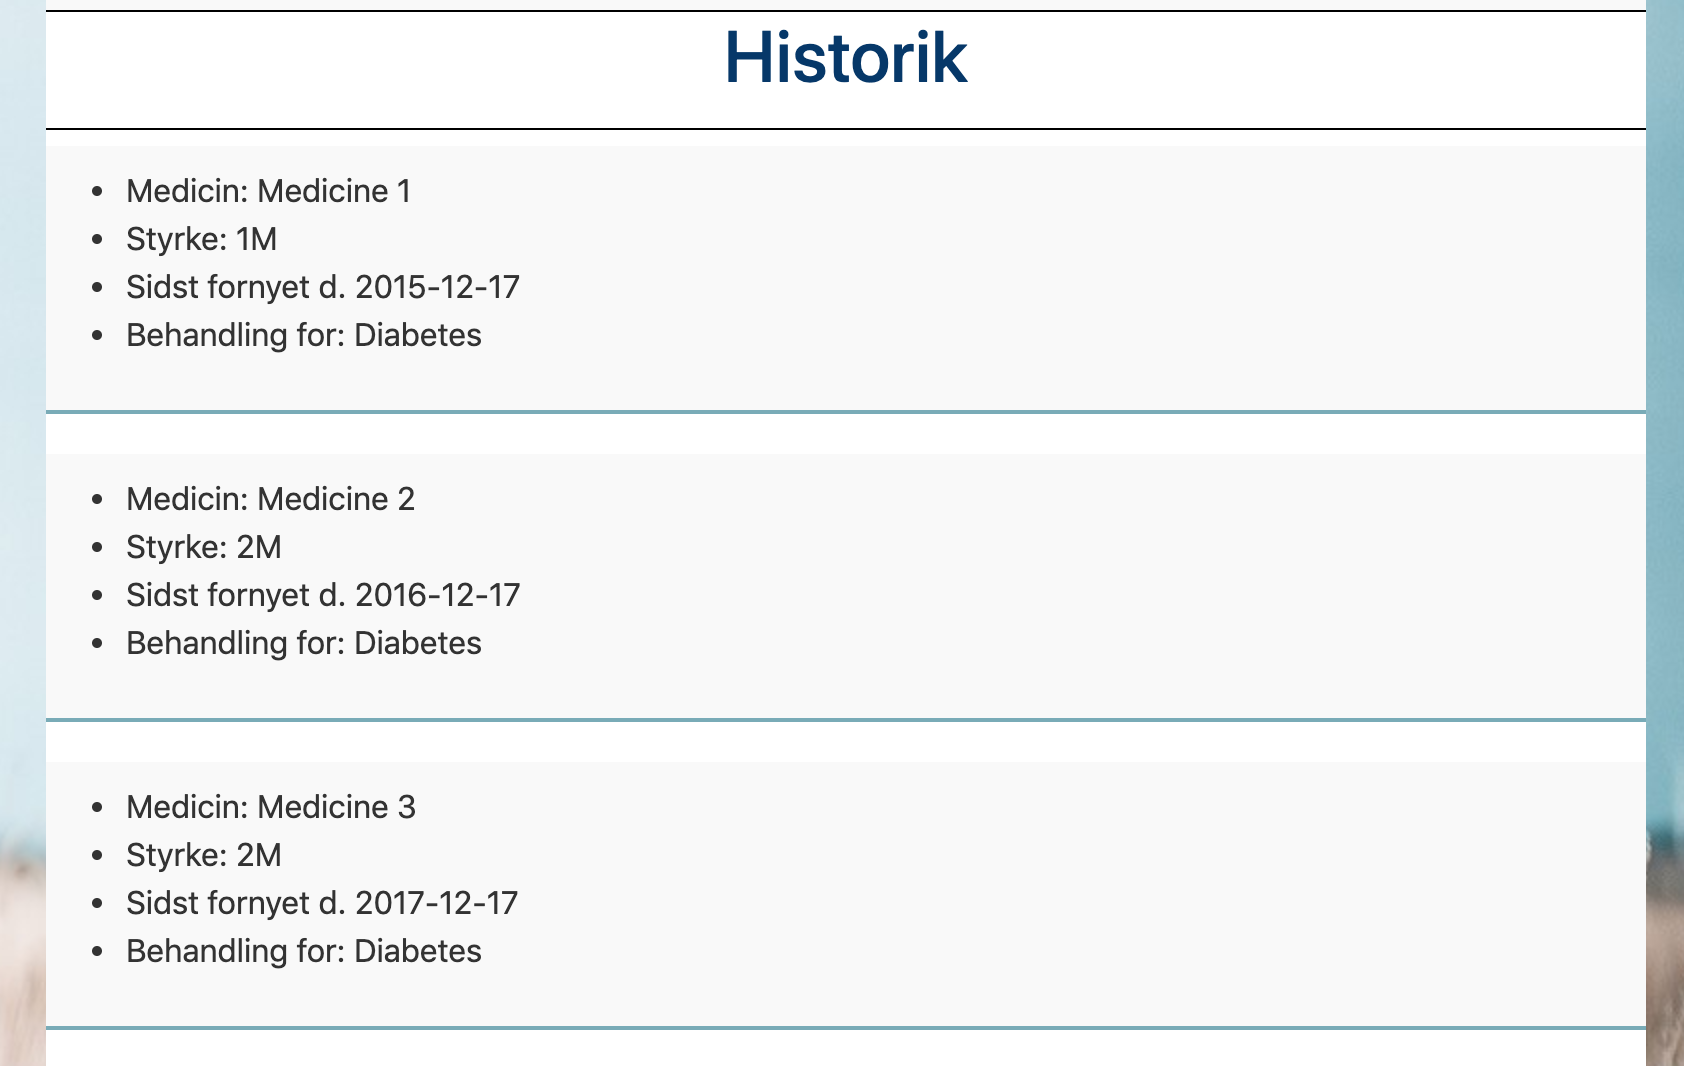
\includegraphics[width=0.49\linewidth]{Materials/Prototype/Historik}
	
\includegraphics[width=0.49\linewidth]{Materials/Prototype/Historik2}
	\caption{tv. ses historikken for brugeren med cprnr. 5000 og th. ses historikken for brugeren med cprnr. 1000}
\end{figure}

Vores prototype består hovedsagligt af tre funktionaliteter: \textit{Receptfornyelse, Historik} og \textit{Sundhedsdata}
\textcolor{red}{S: Sundhedsdata - ? Mener du Medicinkort, eller hvad referer du til?}
. Under \textit{Historik} er det muligt at se alle ens recepter og tidligere recepter, samt information omkring, hvornår recepten blev udskrevet, hvornår den udløb og hvilken medicin, der blev udskrevet.\\
Under \textit{Receptfornyelse} kan alle ens aktive recepter ses. Øverst på siden er en processlinje som beskriver, hvor langt i 'forløbet' ens medicin er kommet, altså om medicinen f.eks. først lige er blevet bestilt, om lægen har godkendt receptfornyelsen, om medicinen kan afhentes, mm. Denne processlinje understøtter vores vision om, at brugeren skal indrages i forløbet og selv kan se fremskridtene i processen. Nedenunder ses de aktive recepter samt en knap, som tillader at fornye recepten. Når brugeren klikker 'forny' ud fra en af sine recepter, så opdateres recepten til ikke længere at være aktiv, og der bliver i stedet lavet en ny recept. I prototypen er de fleste af værdierne i den nye recept hard coded, men dette ville nemt kunne gøres mere realistisk ved at lave om i vores database model.
\begin{figure}[h!]
	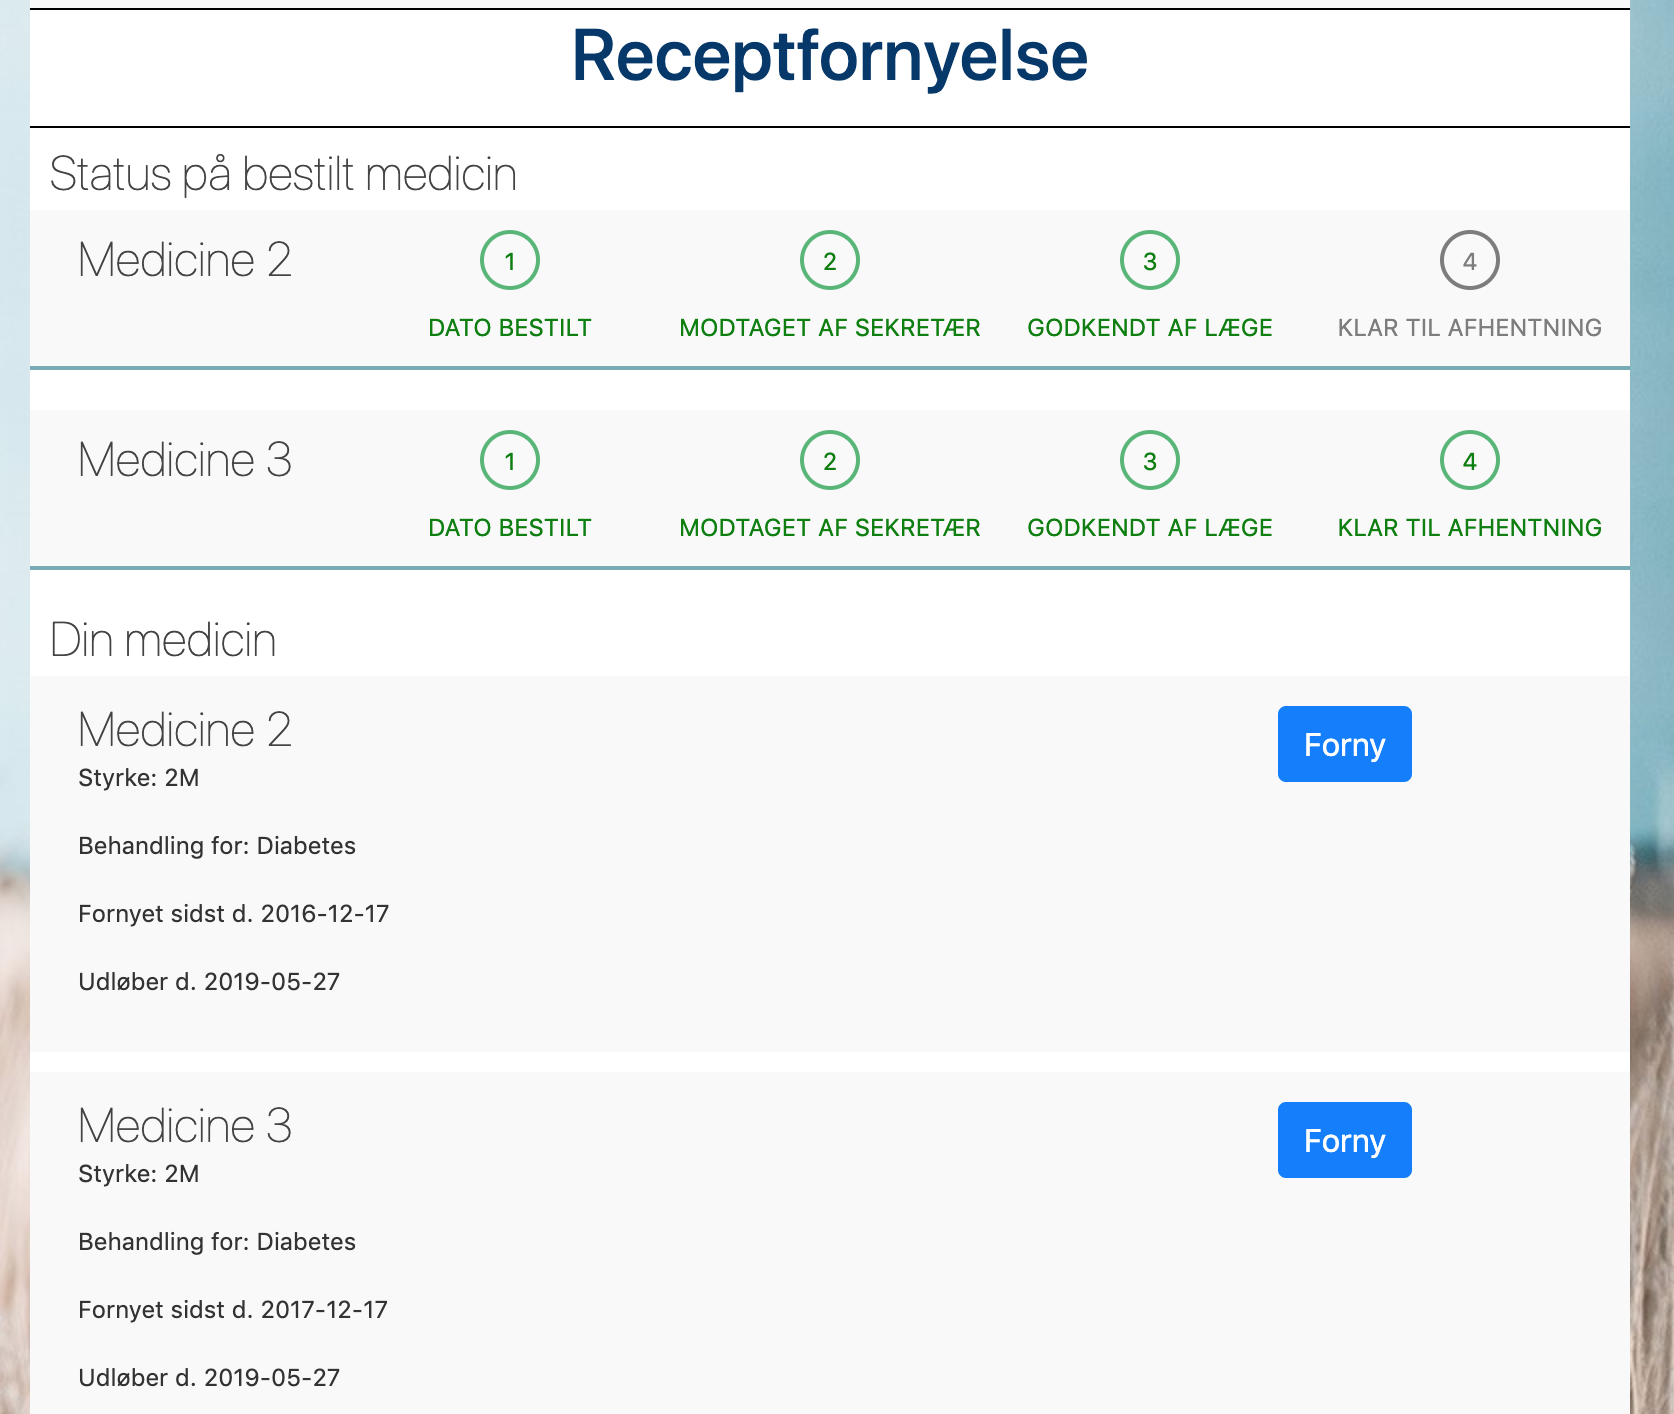
\includegraphics[width=0.49\linewidth]{Materials/Prototype/Receptfornyelse}
	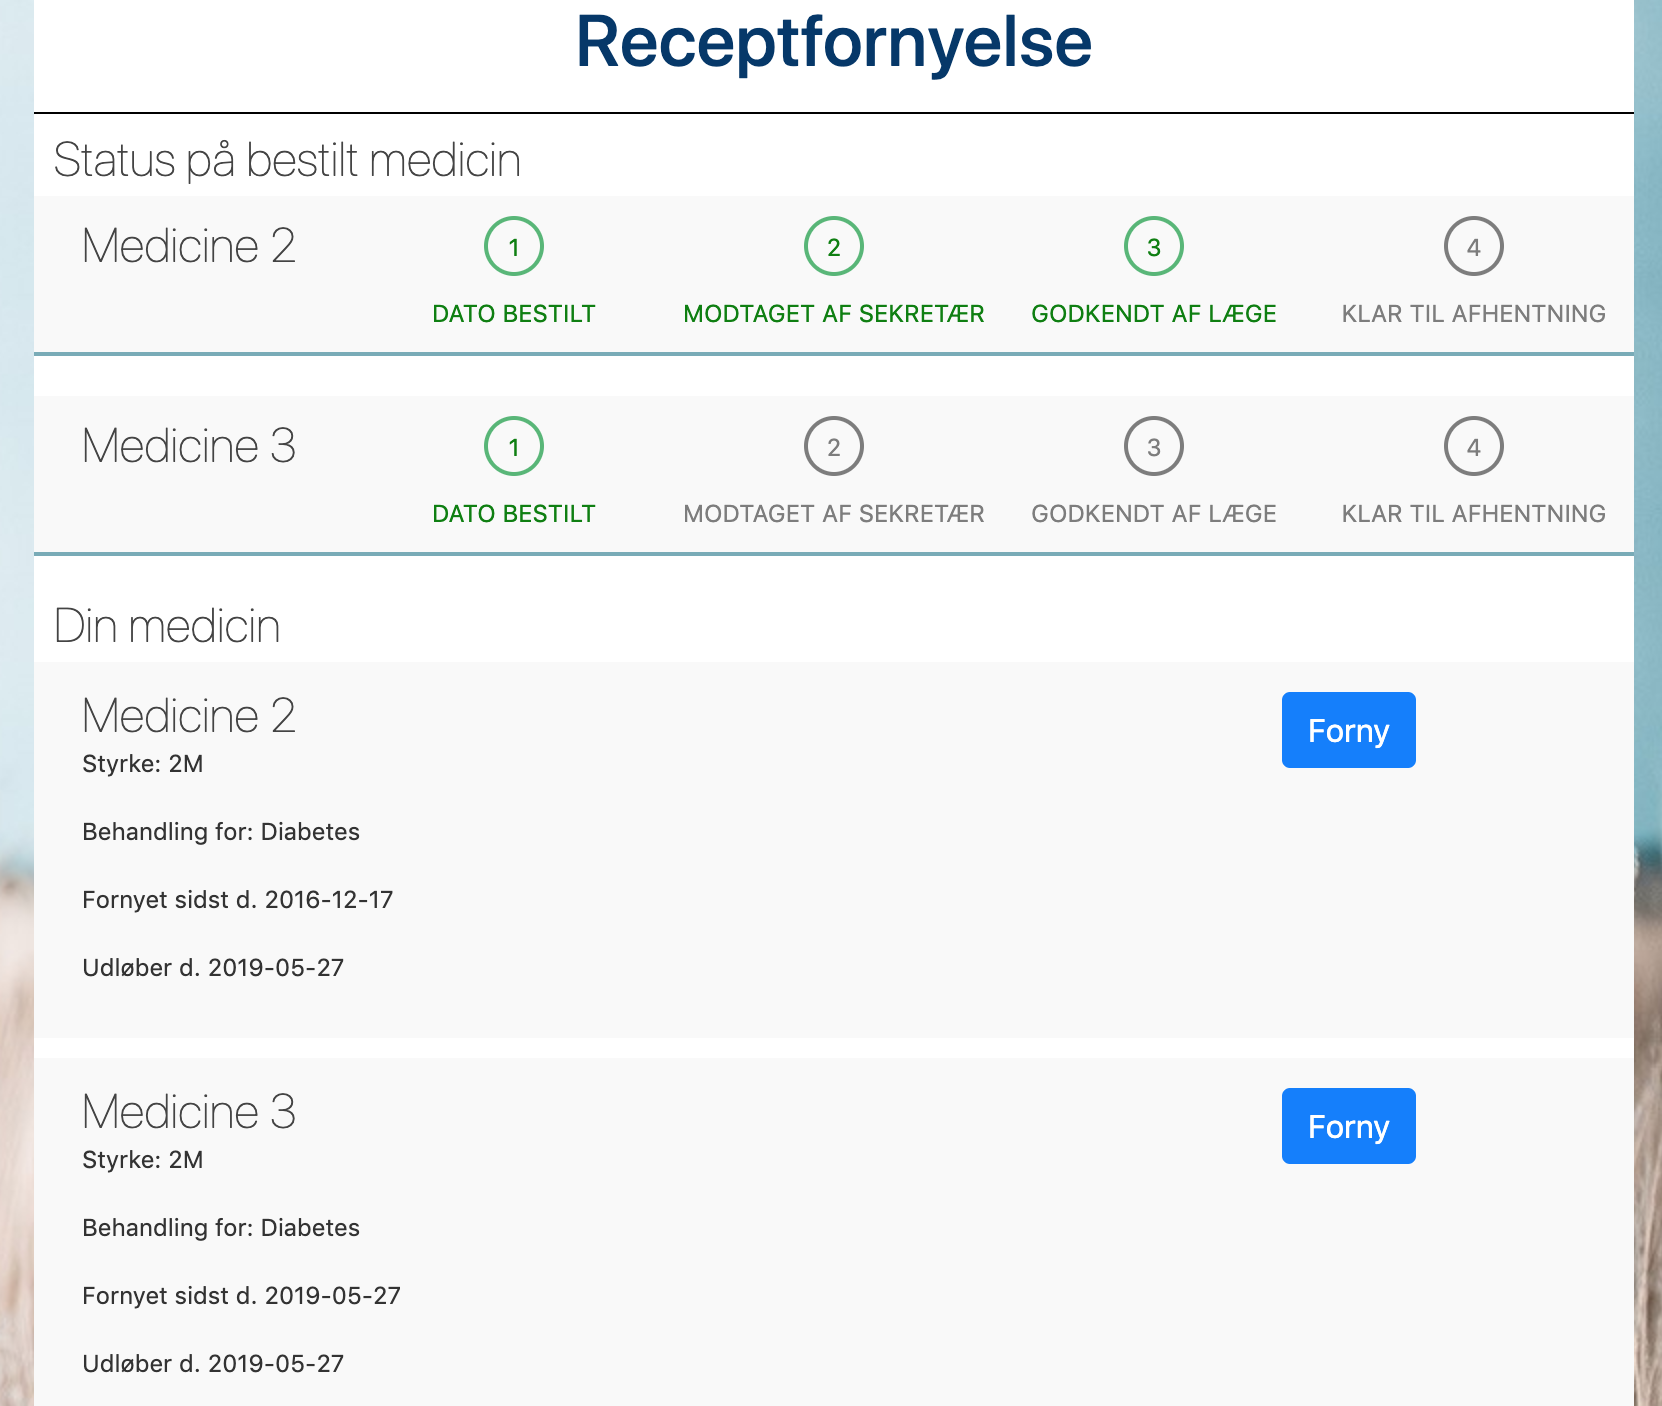
\includegraphics[width=0.49\linewidth]{Materials/Prototype/ReceptfornyelseFornyet}
	\caption{tv. ses recepterne før fornyelse. th. ses recepterne efter 'Medicine 3' fornyelse}
\end{figure}
\newpage
Under \textit{Medicinkort} er det muligt at se alle ens aktive recepter, samt information omkring, hvilken medicin, patienter tager, dens styrke, hvad patienten er i behandling for samt et link til patienthåndbogen for denne diagnose.
\begin{figure}[h!]
	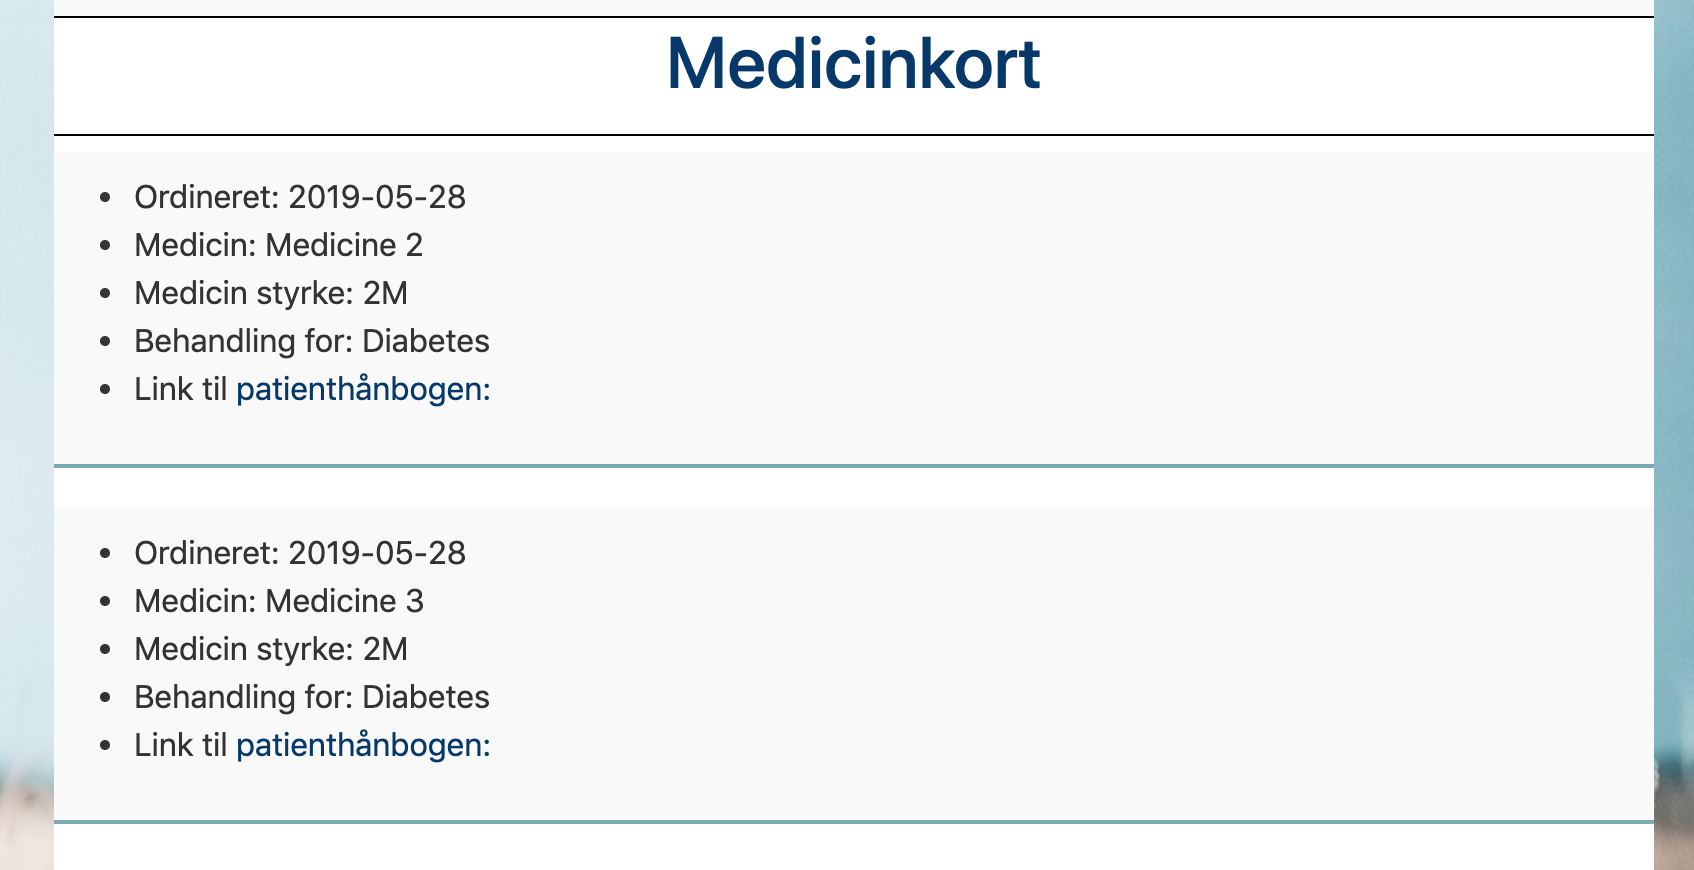
\includegraphics[width=\linewidth]{Materials/Prototype/medicinkort}
	\caption{Medicinkort for brugeren med cprnr. 5000}
\end{figure}
